\documentclass[a4paper, 12pt]{article}

% Essential Packages
\usepackage{amsmath}
\usepackage{amssymb}
\usepackage[top=25mm, bottom=25mm, left=25mm, right=25mm]{geometry}
\usepackage{pgfplots}
\usepackage[inline]{enumitem}
\usepackage{mathtools}
\usepackage{tikz}
\usepackage{fancyhdr}
\usepackage{setspace}
\usepackage{hyperref}

% Misc
\pgfplotsset{compat=1.18}
\usepgfplotslibrary{polar}
\usepgfplotslibrary{fillbetween}
\setlength{\parskip}{3pt}
\setstretch{1.15}
\renewcommand{\headrulewidth}{0pt}
\renewcommand{\footrulewidth}{0pt}
\fancyhf{}

\usepackage{cancel}

\begin{document}
\pagestyle{empty}

\begin{center}
\textbf{2021-2022 Fall\\MAT123 Final\\07/01/2022}
\end{center}

\begin{enumerate}[leftmargin=*,label=\textbf{\arabic*.}]
\item \begin{enumerate}[leftmargin=*,label=\textbf{\alph*.}]
\item Find $\displaystyle\int\frac{dx}{x^3-4x^2+3x}$.

\item Evaluate $\displaystyle\lim_{x\to\textstyle\frac\pi2}\frac{\displaystyle\int_{\pi/2}^x\ln(\sin t)\,dt}{\sin x-1}$.

\item Evaluate the improper integral  $\displaystyle\int_1^2\frac{dx}{(x-1)^{2/3}}$.
\end{enumerate}

\item Consider the region $R$ bounded by the curves $y=\arctan x,\:y=\ln x$ and the lines $\displaystyle x=\frac1{\sqrt3}$ and $x=1$.

\begin{enumerate}[leftmargin=*,label=\textbf{\alph*.}]
\item Find the area of the region $R$. 

\item Write a definite integral (do not evaluate) by using the Washer Method, which gives the volume of a solid obtained by rotating the region $R$ about the $y$-axis.

\item Write a definite integral (do not evaluate) by using the Cylindrical Shell Method, which gives the volume of a solid obtained by rotating the region $R$ about the line $y=2$.
\end{enumerate}

\item Determine whether each series is convergent or divergent. Explain your answer.
\begin{enumerate}[leftmargin=*,label=\textbf{\alph*.}]
\item $\displaystyle\sum_{n=1}^\infty\left(\arctan n-\arctan(n-1)\right)$
\item $\displaystyle\sum_{n=0}^\infty\frac{(-3)^{n+1}}{2^{3n}}$
\item $\displaystyle\sum_{n=1}^\infty\cos\left(\frac{n^2}{1+n^4}\right)$
\item $\displaystyle\sum_{n=2}^\infty\frac1{n(\ln n)^2}$
\end{enumerate}
\end{enumerate}

\newpage
\pagestyle{fancy}
\renewcommand{\headrulewidth}{1pt}
\fancyhead[R]{\textit{2021-2022 Fall Final}}
\fancyhead[L]{\textit{Hacettepe MAT123 Exam Solutions Version 2}}

% Last update: 06/09/2026 15:22

\begin{enumerate}[leftmargin=*,label=\textbf{\arabic*.}]

\item \begin{enumerate}[leftmargin=*,label=\textbf{\alph*.}]
\item Use the method of partial fraction decomposition.
\[\int\frac{dx}{x^3-4x^2+3x}=\int\frac{dx}{x(x-3)(x-1)}=\int\left(\frac Ax+\frac B{x-3}+\frac C{x-1}\right)\,dx\]
\[\begin{array}{rc}A(x-3)(x-1)+Bx(x-1)+Cx(x-3)&=1\\x^2(A+B+C)+x(-4A-B-3C)+3A&=1\\&\end{array}\]

Equate the coefficients of like terms.
\[\left.\begin{array}{r}
x^2(A+B+C)=0\\
x(-4A-B-3C)=0\\
3A=1
\end{array}\right\}\rightarrow A=\frac13,\quad\left.\begin{array}{r}
B+C=-\dfrac13\\[1em]
B+3C=-\dfrac43
\end{array}\right\}\rightarrow B=\frac16,\quad C=-\frac12\]

Rewrite the integral.
\begin{align*}
\int\left(\frac Ax+\frac B{x-3}+\frac C{x-1}\right)\,dx&=\int\left(\frac1{3x}+\frac1{6(x-3)}-\frac1{2(x-1)}\right)\,dx\\[1em]&=\boxed{\frac13\ln|x|+\frac16\ln|x-3|-\frac12\ln|x-1|+c,\quad c\in\mathbb{R}}
\end{align*}

\item The limit is in the indeterminate form $0/0$. Apply L'Hôpital's rule to eliminate the indeterminate form.
\[\lim_{x\to\textstyle\frac\pi2}\frac{\displaystyle\int_{\pi/2}^x\ln(\sin t)\,dt}{\sin x-1}\overset{\text{L'H.}}{=}\lim_{x\to\textstyle\frac\pi2}\frac{\displaystyle\frac d{dx}\int_{\pi/2}^x\ln(\sin t)\,dt}{\cos x}\]

By the Fundamental Theorem of Calculus, we may rewrite the limit as follows.
\begin{align*}\lim_{x\to\textstyle\frac\pi2}\frac{\displaystyle\frac d{dx}\int_{\pi/2}^x\ln(\sin t)\,dt}{\cos x}&=\lim_{x\to\textstyle\frac\pi2}\frac{\ln(\sin x)}{\cos x}\overset{\text{L'H.}}{=}\lim_{x\to\textstyle\frac\pi2}\frac{\frac1{\sin x}\cdot\cos x}{-\sin x}\\[1em]&=\lim_{x\to\textstyle\frac\pi2}\frac{\cos x}{-\sin^2x}=-\frac{\cos\frac\pi2}{\sin^2\frac\pi2}=\boxed0\end{align*}

\item Take the limit since this is an improper integral.
\begin{align*}
\int_1^2\frac{dx}{(x-1)^{2/3}}
&=\lim_{R\to1^+}\int_R^2\frac{dx}{(x-1)^{2/3}}
=\lim_{R\to1^+}3(x-1)^{1/3}\bigg|_R^2\\[1em]
&=3\lim_{R\to1^+}\left(1-(R-1)^{1/3}\right)
=\boxed{3}
\end{align*}
\end{enumerate}

\newpage
\item\leavevmode
\vspace{-1.5em}
\begin{center}
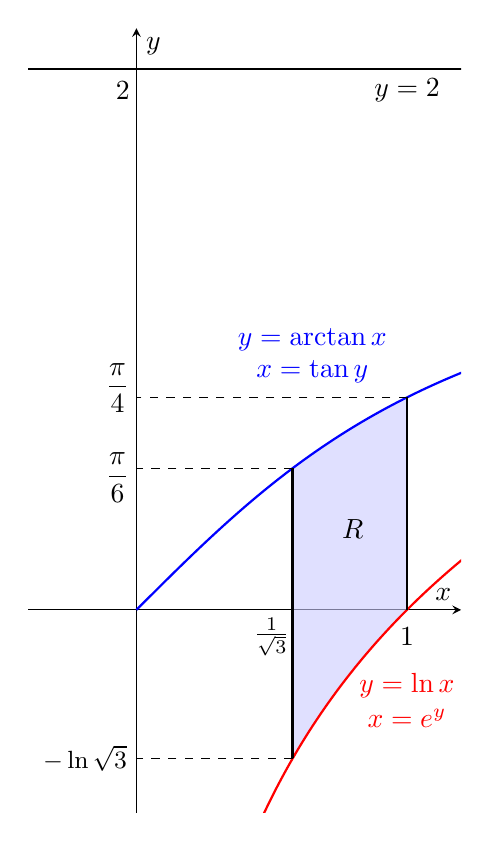
\begin{tikzpicture}
  \begin{axis}[
      axis lines=center,
      axis equal image,
      xlabel={$x$},
      ylabel={$y$},
      xmin=-0.4, xmax=1.2,
      ymin=-0.75, ymax=2.15,
      samples=200,
      scale=1.75,
      domain=0.577:1,
      xtick=\empty, ytick=\empty,
    ]

    \addplot [thick, blue, name path=A, domain=0:2] {rad(atan(x))};
    \addplot [thick, red, name path=B, domain=0.1:2] {ln(x)};
    \addplot [blue!20, fill opacity=0.6] fill between[of=A and B,soft clip={domain=0.577:1}];
    
    \draw[dashed] (-3,0) -- (-3,3); \draw[dashed] (-3,3) -- (-0.5,3);
    \draw[dashed] (2,0) -- (2,8); \draw[dashed] (0,8) -- (2,8);

    \node[blue] at (0.65,1) {$y=\arctan x$}; \node[blue] at (0.65,0.88) {$x=\tan y$};
    \node[red] at (1,-0.28) {$y=\ln x$}; \node[red] at (1,-0.4) {$x= e^y$};

    \draw[thick] (0.577,-0.549)--(0.577,0.523); \draw[thick] (1,0)--(1,0.785);
    \draw[dashed] (1,0.785)--(0,0.785); \draw[dashed] (0.577, 0.523)--(0,0.523);
    \draw[dashed] (0.577,-0.549)--(0,-0.549);
    \draw[thick] (-1,2)--(2,2); 
    
    \node at (0.8,0.3) {$R$}; \node at (0.5,-0.1) {$\frac1{\sqrt3}$}; \node at (-0.07,0.49) {$\dfrac\pi6$}; \node at (-0.07,0.82) {$\dfrac\pi4$}; \node at (-0.19,-0.549) {\small $-\ln\sqrt3$}; \node at (1,-0.1) {$1$}; \node at (-0.05,1.92) {$2$}; \node at (1,1.92) {$y=2$};
\end{axis}
\end{tikzpicture}
\end{center}

\begin{enumerate}[leftmargin=*,label=\textbf{\alph*.}]
\item Set up the integral.
\begin{equation}A=\int_{1/\sqrt3}^1\left(\arctan x-\ln x\right)\,dx=\int_{1/\sqrt3}^1\arctan x\,dx-\int_{1/\sqrt3}^1\ln x\,dx\label{eq:21_22_fall_final_1}\end{equation}

Calculate the first integral in \eqref{eq:21_22_fall_final_1} by integration by parts.
\[\left.\begin{array}{c}
u=\arctan x\implies du=\dfrac1{x^2+1}\,dx\\[1em]
dv=dx\implies v=x
\end{array}\right\}\rightarrow \int u\,dv=uv-\int v\,du\]
\begin{align*}\int_{1/\sqrt3}^1\arctan x\,dx&=x\arctan x\bigg|_{1/\sqrt3}^1-\int_{1/\sqrt3}^1\frac{x}{x^2+1}\,dx\\[1em]&=\left(x\arctan x-\frac12\ln\left|x^2+1\right|\right)\Bigg|_{1/\sqrt3}^1\\[1em]&=\left(\frac\pi4-\frac{\ln 2}2\right)-\left(\frac{\pi\sqrt3}{18}-\frac12\ln\left(\frac43\right)\right)=\frac{\pi\left(9-2\sqrt3\right)}{36}+\frac12\ln\frac23\end{align*}

Calculate the second integral in\eqref{eq:21_22_fall_final_1} by integration by parts.
\[\left.\begin{array}{c}
u=\ln x\implies du=\dfrac1x\,dx\\[1em]
dv=dx\implies v=x
\end{array}\right\}\rightarrow \int u\,dv=uv-\int v\,du\]
\begin{align*}\int_{1/\sqrt3}^1\ln x\,dx&=x\ln x\bigg|_{1/\sqrt3}^1-\int_{1/\sqrt3}^1\,dx=\left(x\ln x-x\right)\Bigg|_{1/\sqrt3}^1\\[1em]&=\left(0-1\right)-\left(-\frac{\ln\sqrt3}{\sqrt3}-\frac1{\sqrt3}\right)=\frac{\sqrt3\ln\sqrt3+\sqrt3-3}3\end{align*}

The result is then
\[\boxed{A=\frac{\pi\left(9-2\sqrt3\right)}{36}+\frac12\cdot\ln\frac23-\frac{\sqrt3\ln\sqrt3+\sqrt3-3}3}\]

\item\leavevmode
\vspace{-2em}
\begin{align*}\boxed{\begin{array}{l}\displaystyle\int_{-\ln\sqrt3}^0\pi\left[\left( e^y\right)^2-\left(\frac1{\sqrt3}\right)^2\right]\,dy+\int_0^{\pi/6}\pi\left[(1)^2-\left(\frac1{\sqrt3}\right)^2\right]\,dy\\[1em]\displaystyle+\int_{\pi/6}^{\pi/4}\pi\left[(1^2)-\left(\tan y\right)^2\right]\,dy\end{array}}\end{align*}

\item\leavevmode
\vspace{-2em}
\begin{align*}\boxed{\begin{array}{l}\displaystyle\int_{-\ln\sqrt3}^02\pi\left(2-y\right)\left( e^y-\frac1{\sqrt3}\right)\,dy+\int_0^{\pi/6}2\pi\left(2-y\right)\left(1-\frac1{\sqrt3}\right)\,dy\\[1em]\displaystyle+\int_{\pi/6}^{\pi/4}2\pi\left(2-y\right)\left(1-\tan y\right)\,dy\end{array}}\end{align*}
\end{enumerate}

\item
\begin{enumerate}[leftmargin=*,label=\textbf{\alph*.}]
\item Determine the $n$th partial sum.
\begin{align*}\sum_{n=1}^{\infty}\left(\arctan n -\arctan(n-1)\right)&=\left(\cancel{\arctan1}-\arctan0\right)+\left(\cancel{\arctan2}-\cancel{\arctan1}\right)\\&\quad+\left(\cancel{\arctan3}-\cancel{\arctan2}\right)+\left(\cancel{\arctan4}-\cancel{\arctan3}\right)\\[1em]&\quad +\cdots\:+\left(\arctan n-\cancel{\arctan(n-1)}\right)\\[1em]&=\arctan n-\arctan0=\arctan n\end{align*}
\[\lim_{n\to\infty}\arctan n=\frac\pi2\quad(\text{convergent})\]

Therefore, the series $\displaystyle\sum_{n=1}^{\infty}\left(\arctan n -\arctan(n-1)\right)$ $\boxed{\text{converges}}$.

\item Rewrite the sum.
\begin{align*}\sum_{n=0}^{\infty}\frac{(-3)^{n+1}}{2^{3n}}=\sum_{n=0}^{\infty}\frac{-3\cdot(-3)^n}{8^n}=-3\sum_{n=0}^{\infty}\left(-\frac38\right)^n\end{align*}

This is a geometric series where $r=-\dfrac38$. $|r|=\dfrac38<1$. Therefore, the series $\displaystyle\sum_{n=0}^{\infty}\frac{(-3)^{n+1}}{2^{3n}}$ converges.

\item Apply the $n$th Term Test for divergence. We may take the limit inside the trigonometric function because $\cos x$ is continuous everywhere. Since $1+n^4$ grows faster than $n^2$, the value of the expression $\dfrac{n^2}{1+n^4}$ tends to zero.
\[\lim_{n\to\infty}\cos\left(\frac{n^2}{1+n^4}\right)=\cos\left[\lim_{n\to\infty}\left(\frac{n^2}{1+n^4}\right)\right]=\cos0=1\neq0\]

By the $n$th Term Test for divergence, the series $\displaystyle\sum_{n=1}^\infty\cos\left(\frac{n^2}{1+n^4}\right)$ diverges.

\item Take $\displaystyle f(x)=\frac1{x(\ln x)^2}$. $f$ is positive and decreasing for $x\geq2$ because $x$ and $(\ln x)^2$ are positive and increasing for $x\geq2$. $x$ is a polynomial which is defined everywhere and $(\ln x)^2$ is continuous for $x\geq2$. Since we took into account every criterion, we may apply the Integral Test. Handle the improper integrals by taking the limit.
\[\int_2^{\infty}\frac{dx}{x(\ln x)^2}=\lim_{R\to\infty}\int_2^R\frac{dx}{x(\ln x)^2}=\lim_{R\to\infty}\left[-\frac1{\ln x}\right]_2^R=\lim_{R\to\infty}\left[-\frac1{\ln R}+\frac1{\ln2}\right]=\frac1{\ln 2}\]

Since the integral converges, the series $\displaystyle\sum_{n=2}^\infty\frac1{n(\ln n)^2}$ also converges.
\end{enumerate}
\end{enumerate}
\end{document}